%%%%%%%%%%%%%%%%%%%%%%%%%%%%%%%%%%%%%%%%%%%%%%%%%%%%%%%%%%%%%%%%%%%%%%%%%%%%%%%%
% Audio
%%%%%%%%%%%%%%%%%%%%%%%%%%%%%%%%%%%%%%%%%%%%%%%%%%%%%%%%%%%%%%%%%%%%%%%%%%%%%%%%
\chapter{Audio} \label{Audio}
\vspace{-10ex}\mAu{syml}\vskip 8ex

%%%%%%%%%%%%%%%%%%%%%%%%%%%%%%%%%%%%%%%%%%%%%%%%%%%%%%%%%%%%%%%%%%%%%%%%%%%%%%%%
% Introduction
%%%%%%%%%%%%%%%%%%%%%%%%%%%%%%%%%%%%%%%%%%%%%%%%%%%%%%%%%%%%%%%%%%%%%%%%%%%%%%%%
\section{Introduction}

The left side of the front panel is devoted to \mAu{f} playback and control.
Its functionality is available at all times independent of any mode the device
may be in.\footnote{ One exception is during touch calibration - see
\hyperref[Touch Settings]{\mTS{ss}}.}

\begin{itemize}
  \item It can \sAuPl{f} and \sAuPa{f} the audio files stored on the removable
    \cMSD{f} attached to the circuit board.
  \item You can \sAuSt{f} it for extra power savings when running unplugged.
  \item It can \sAuSk{f} forward or backward tracks or rewind the current track.
\end{itemize}

\info{The \cDi{f} is \textit{not} capable of
displaying the track \textit{name} being played so track
\textit{numbers}\footnote{ The numbers represent the order on disk and not any
kind of album track order.} are displayed instead when applicable.}

There is an auto-stop feature that can be enabled via
\hyperref[Power Settings]{\mPS{f}}.  If in the \sAuPa{f} state for a
configurable amount of time, the \mAu{f} will automatically turn off
and go into the \sAuSt{f} state.

%%%%%%%%%%%%%%%%%%%%%%%%%%%%%%%%%%%%%%%%%%%%%%%%%%%%%%%%%%%%%%%%%%%%%%%%%%%%%%%%
% Volume
%%%%%%%%%%%%%%%%%%%%%%%%%%%%%%%%%%%%%%%%%%%%%%%%%%%%%%%%%%%%%%%%%%%%%%%%%%%%%%%%
\section{Volume} \label{Audio - Volume}

The \cVo{f} knob controls the volume level of the \mAu{f}\footnote{ The
\cVo{ss} is not connected to the \cBe{ss} so cannot control its volume.}
and has a \textit{white arrow} indicator on the sleeve.  Unlike the \cEs{f} and
\cBr{f} it does \textit{not} turn indefinitely and stops at the
\textit{minimum} and \textit{maximum} positions as indicated below.

\begin{itemize}
  \item Turn \textit{clockwise} to \textit{increase} the volume.
  \item Turn \textit{counter-clockwise} to \textit{decrease} the volume.
\end{itemize}

\begin{table}[H]
\ers{1}
\centering
\begin{tabular}{ c c c }
  Minimum & Adjust & Maximum \\
  \includegraphics{images/volume_lo.png}
    & 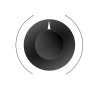
\includegraphics{images/volume.png}
    & 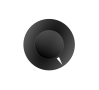
\includegraphics{images/volume_hi.png}
\end{tabular}
\caption{Volume Control}
\end{table}

%%%%%%%%%%%%%%%%%%%%%%%%%%%%%%%%%%%%%%%%%%%%%%%%%%%%%%%%%%%%%%%%%%%%%%%%%%%%%%%%
% Symbols
%%%%%%%%%%%%%%%%%%%%%%%%%%%%%%%%%%%%%%%%%%%%%%%%%%%%%%%%%%%%%%%%%%%%%%%%%%%%%%%%
\section{Symbols}  \label{Audio - Symbols}

There are a number of symbols that will be used in the next sections to
describe the controls and actions that can be performed.

\ers{2.8}
\begin{longtabu}{ X[1,c,m] | X[4,l,m] }
  \thrule
  \multicolumn{2}{c}{\thb{Controls}} \\ \mrule
  \thbi{Symbol} & \thbi{Description} \\ \mrule

  \sPl & \cPl{f} push-button. \\ \drule{2}
  \sNe & \cNe{f} push-button. \\ \drule{2}
  \sPr & \cPr{f} push-button. \\ \thrule

  \multicolumn{2}{c}{\thb{Actions}} \\ \mrule
  \thbi{Symbol} & \thbi{Description} \\ \mrule

  \sPlay
    & Press \& Release \thinspace\sPl\enspace to \sAuPl{f} the \mAu{f}
      when it is in the \sAuPa{f} or \sAuSt{f} states. \\ \drule{2}
  \sPause
    & Press \& Release \thinspace\sPl\enspace to \sAuPa{f} the \mAu{f}
      when it is in the \sAuPl{f} state. \\ \drule{2}
  \sStop
    & Press \& Hold \thinspace\sPl\enspace until \symD{StOP}
      is displayed then release to \sAuSt{f} the \mAu{f}
      when it is in the \sAuPl{f} or \sAuPa{f} states. \\ \drule{2}
  \sNext
    & Press \& Release or Press \& Hold \thinspace\sNe\enspace to \sAuSk{f}
      forward tracks. \\ \drule{2}

  \pagebreak \drule{2}
  \sPrev
    & Press \& Release or Press \& Hold \thinspace\sPr\enspace to \dRe{f}
      the current track or \sAuSk{f} backward tracks. \\

  \bhrule
\caption{Audio Symbols}
\end{longtabu}

%%%%%%%%%%%%%%%%%%%%%%%%%%%%%%%%%%%%%%%%%%%%%%%%%%%%%%%%%%%%%%%%%%%%%%%%%%%%%%%%
% Play|Pause|Stop
%%%%%%%%%%%%%%%%%%%%%%%%%%%%%%%%%%%%%%%%%%%%%%%%%%%%%%%%%%%%%%%%%%%%%%%%%%%%%%%%
\section{Play | Pause | Stop} \label{Audio - Play|Pause|Stop}

The \thinspace\sPl\enspace push-button can \sAuPl{f}, \sAuPa{f} or \sAuSt{f}
the \mAu{f}.

\par\medskip

The \mAu{f} starts in the \sAuSt{f} state when the device is initially switched
\sOn{f} via the \cPo{f}.  To start playback, \aPR{f}.

\ase{1}{{c c c c}}{%
\sAuSt{sym} & \sPlay & \eStart{sym}{PLAYBACK} & \sAuPl{sym} \\}

To \sAuPa{f}, \aPR{f} when in the \sAuPl{f} state.

\ase{1}{{c c c c}}{%
\sAuPl{sym} & \sPause & \ePa{sym}{PLAYBACK} & \sAuPa{sym} \\}

To resume playback, \aPR{f} when in the \sAuPa{f} state.

\ase{1}{{c c c c}}{%
\sAuPa{sym} & \sPlay & \eResume{sym}{PLAYBACK} & \sAuPl{sym} \\}

To \sAuSt{f} the \mAu{f} when in \sAuPl{f} or \sAuPa{f} states, \aPH{f} for
\mono{2} seconds and \aRe{f} when the \cDi{f} shows

\begin{figure}[H]
\centering
  \sDl{StOP}
\end{figure}

\ase{1}{{c c c c}}{%
\sAuPl{sym} & \multirow{2}{*}{\sStop} & \multirow{2}{*}{\eSt{sym}{PLAYBACK}}
  & \multirow{2}{*}{\sAuSt{sym}} \\ \dcrule{1}{1}
\sAuPa{sym} & & & \\}

Besides the power savings that \sAuSt{f} provides over \sAuPa{f},
there is another difference between \sAuPa{f} and \sAuSt{f}.

\begin{itemize}
  \item When resuming from \sAuPa{f}, the the track will resume playing from
    the same place as when it was paused.
  \item When resuming from \sAuSt{f}, the track will start playing from the
    beginning.
\end{itemize}

%%%%%%%%%%%%%%%%%%%%%%%%%%%%%%%%%%%%%%%%%%%%%%%%%%%%%%%%%%%%%%%%%%%%%%%%%%%%%%%%
% Next
%%%%%%%%%%%%%%%%%%%%%%%%%%%%%%%%%%%%%%%%%%%%%%%%%%%%%%%%%%%%%%%%%%%%%%%%%%%%%%%%
\section{Next} \label{Audio - Next}

The \thinspace\sNe\enspace push-button is used to \aSkip{f} \textit{forward}
one or more tracks.  

\begin{itemize}
  \item \aPR{f} to \aSkip{f} to the \textit{next} track.
    \begin{itemize}
      \item The next track number will \textit{not} be shown on the \cDi{f}.
    \end{itemize}
  \item \aPH{f} to \aSkip{f} \textit{forward} one or more tracks.
    \begin{itemize}
      \item The longer the push-button is held, the faster tracks will progress.
      \item The track numbers \textit{will} be shown on the \cDi{f}, for
        example:
        \figD{!!22}{Track \#22}
      \item \aRe{f} when you get to the track you want.
    \end{itemize}
\end{itemize}

\as{{c c c c c}}{%
\sAuPl{sym} & & & & \\ \dcrule{1}{1}
\sAuPa{sym} & \sNext & \sAuSk{sym} & \eSk{sym}{FORWARD} & \sAuPl{sym} \\ \dcrule{1}{1}
\sAuSt{sym} & & & & \\}

\begin{table}[H]
\ers{1}
\centering
\begin{tabu} { X[1,c,m] | X[1,c,m] }
  \thrule
  \thbi{Hold Time} & \thbi{Tracks per Second} \\ \mrule
  First \num{5} Tracks & \num{1} \\ \drule{2}
  Next \num{10} Tracks & \num{2} \\ \drule{2}
  Next \num{20} Tracks & \num{4} \\ \drule{2}
  Next \num{40} Tracks & \num{8} \\ \drule{2}
  Next \num{80} Tracks & \num{16} \\ \drule{2}
  Next \textit{\large\mono{N}} Tracks & \num{32} \\
  \bhrule
\end{tabu}
\caption{Audio - Next Hold Times}
\end{table}

\info{When the device is in the \sPoSl{f} power state, \sNe\enspace
can \textit{not} wake it - see \hyperref[Power]{\mPo{f}} for more
information and controls that can wake the device from \sPoSl{f}.}

%%%%%%%%%%%%%%%%%%%%%%%%%%%%%%%%%%%%%%%%%%%%%%%%%%%%%%%%%%%%%%%%%%%%%%%%%%%%%%%%
% Previous
%%%%%%%%%%%%%%%%%%%%%%%%%%%%%%%%%%%%%%%%%%%%%%%%%%%%%%%%%%%%%%%%%%%%%%%%%%%%%%%%
\section{Previous} \label{Audio - Previous}

The \thinspace\sPr\enspace push-button is used to \aSkip{f} \textit{backward}
one or more tracks or \dRe{f} the current track.

\begin{itemize}
  \item \aPR{f}
    \begin{itemize}
      \item \dRe{f} the current track if more than $\frac{1}{4}$ of the track
        has played.
      \item Otherwise, \aSkip{f} to the \textit{previous} track.
      \item The track number will \textit{not} be shown on the \cDi{f}.
    \end{itemize}
  \item \aPH{f} to \aSkip{f} \textit{backward} one or more tracks.
    \begin{itemize}
      \item The longer the push-button is held, the faster tracks will progress.
      \item The track numbers \textit{will} be shown on the \cDi{f}, for example:
        \figD{!!!8}{Track \#8}
      \item \aRe{f} when you get to the track you want.
    \end{itemize}
\end{itemize}

\as{{c c c c c}}{%
\sAuPl{sym} & \multirow{3}{*}[-1.5mm]{\sPrev} & \multirow{3}{*}[-1.5mm]{\sAuSk{sym}}
  & \multirow{3}{*}[-2.5mm]{%
    \begin{tabu}{c} \eRewind{sym}{CURRENT TRACK} \\ \drule{1} \eSk{sym}{BACKWARD} \end{tabu}}
  & \multirow{3}{*}{\sAuPl{sym}} \\ \dcrule{1}{1}
\sAuPa{sym} & & & & \\ \dcrule{1}{1}
\sAuSt{sym} & & & & \\}

\begin{table}[H]
\ers{1}
\centering
\begin{tabu}{ X[1,c,m] | X[1,c,m] }
  \thrule
  \thbi{Hold Time} & \thbi{Tracks per Second} \\ \mrule
  First \num{5} Tracks & \num{1} \\ \drule{2}
  Next \num{10} Tracks & \num{2} \\ \drule{2}
  Next \num{20} Tracks & \num{4} \\ \drule{2}
  Next \num{40} Tracks & \num{8} \\ \drule{2}
  Next \num{80} Tracks & \num{16} \\ \drule{2}
  Next \textit{\large\mono{N}} Tracks & \num{32} \\
  \bhrule
\end{tabu}
\caption{Audio - Previous Hold Times}
\end{table}

\info{When the device is in the \sPoSl{f} power state, \sPr\enspace
can \textit{not} wake it - see \hyperref[Power]{\mPo{f}} for more
information and controls that can wake the device from \sPoSl{f}.}

%%%%%%%%%%%%%%%%%%%%%%%%%%%%%%%%%%%%%%%%%%%%%%%%%%%%%%%%%%%%%%%%%%%%%%%%%%%%%%%%
% Track Selection
%%%%%%%%%%%%%%%%%%%%%%%%%%%%%%%%%%%%%%%%%%%%%%%%%%%%%%%%%%%%%%%%%%%%%%%%%%%%%%%%
\section{Track Selection} \label{Audio - Track Selection}

In addition to using the \cNe{f} and \cPr{f} controls to \sAuSk{f} forward and
backward in order to select a track for playback, there also exists the
capability to select a track more quickly and directly when in
\hyperref[Clock]{\mCl{f}} mode.  The \cEs{f} can be used alone or in
combination with \aTo{f} to do so.  Refer to \hyperref[Show Track]{Show Track}
and \hyperref[Set Track]{Set Track} in that section for more information.

%%%%%%%%%%%%%%%%%%%%%%%%%%%%%%%%%%%%%%%%%%%%%%%%%%%%%%%%%%%%%%%%%%%%%%%%%%%%%%%%
% Reference
%%%%%%%%%%%%%%%%%%%%%%%%%%%%%%%%%%%%%%%%%%%%%%%%%%%%%%%%%%%%%%%%%%%%%%%%%%%%%%%%
\section{Reference} \label{Audio - Reference}

\ers{2}
\begin{longtabu}{ X[2,c,m] | X[2,c,m] | X[2,c,m] | X[4,c,m] | X[2,c,m] }
  \thrule

  \thbi{State} & \thbi{Action} & \thbi{Control} & \thbi{Effect} & \thbi{Next} \\ \mdrule

  \multirow{3}{*}[-1.5mm]{\sAuSt{sym}}
    & \sPlay & \sPl & \ePl{sym}{AUDIO} & \sAuPl{sym} \\ \dcrule{2}{5}
  & \sNext & \sNe & \eSk{sym}{FORWARD}
    & \multirow{2}{*}[-1mm]{\sAuSk{sym}} \\ \dcrule{2}{4}
  & \sPrev & \sPr & \eSk{sym}{BACKWARD} & \\ \mrule

  \multirow{4}{*}[-1.5mm]{\sAuPl{sym}}
    & \sPause & \sPl & \ePa{sym}{AUDIO} & \sAuPa{sym} \\ \dcrule{2}{5}
  & \sNext & \sNe & \eSk{sym}{FORWARD}
    & \multirow{2}{*}[-1mm]{\sAuSk{sym}} \\ \dcrule{2}{4}
  & \sPrev & \sPr & \eSk{sym}{BACKWARD} & \\ \dcrule{2}{5}
  & \sStop & \sPl & \eSt{sym}{AUDIO} & \sAuSt{sym} \\ \mrule

  \multirow{5}{*}[-1.5mm]{\sAuPa{sym}}
    & \sPlay & \sPl & \eResume{sym}{AUDIO} & \sAuPl{sym} \\ \dcrule{2}{5}
  & \sNext & \sNe & \eSk{sym}{FORWARD}
    & \multirow{2}{*}[-1mm]{\sAuSk{sym}} \\ \dcrule{2}{4}
  & \sPrev & \sPr & \eSk{sym}{BACKWARD} & \\ \dcrule{2}{5}
  & \sStop & \sPl & \multirow{2}{*}[-1mm]{\eSt{sym}{AUDIO}}
    & \multirow{2}{*}[-1mm]{\sAuSt{sym}} \\ \dcrule{2}{3}
  & \action{ss}{INACTIVITY} & --- & & \\ \mrule

  \multirow{4}{*}[-1mm]{\sAuSk{sym}} & \sNext & \sNe
    & \eSk{sym}{FORWARD} & \multirow{2}{*}[-1mm]{---} \\ \dcrule{2}{4}
  & \sPrev & \sPr & \eSk{sym}{BACKWARD} & \\ \dcrule{2}{5}
  & \multirow{2}{*}[-1mm]{\action{ss}{RELEASE}} & \sNe
    & \multirow{2}{*}[-1mm]{\ePl{sym}{TRACK}}
    & \multirow{2}{*}[-1mm]{\sAuPl{sym}} \\ \dcrule{3}{3}
  & & \sPr & & \\

  \bhrule
\caption {Audio - Reference}
\end{longtabu}

%%%%%%%%%%%%%%%%%%%%%%%%%%%%%%%%%%%%%%%%%%%%%%%%%%%%%%%%%%%%%%%%%%%%%%%%%%%%%%%%
% Audio - State Diagram
%%%%%%%%%%%%%%%%%%%%%%%%%%%%%%%%%%%%%%%%%%%%%%%%%%%%%%%%%%%%%%%%%%%%%%%%%%%%%%%%
\section{State Diagram} \label{Audio - State Diagram}

\begin{figure}[H]
  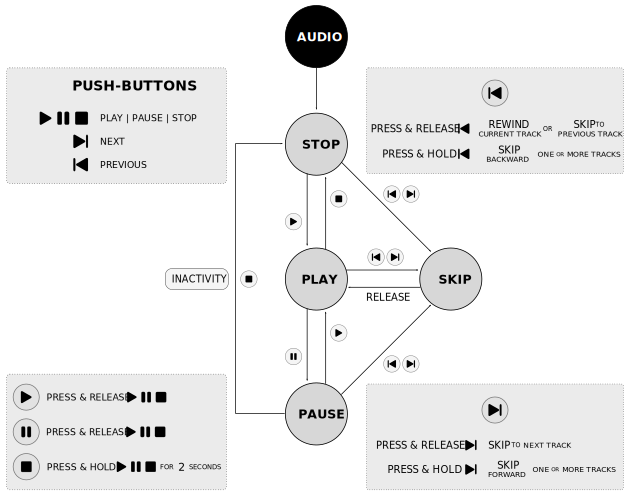
\includegraphics{images/audio_state_diagram.png}
\caption{Audio - State Diagram}
\end{figure}
